% Crofton's formula: a curve and random lines (uniform for the invariant measure among lines meeting a disc); and the Reuleaux triangle between parallel lines. Generated by a short script.
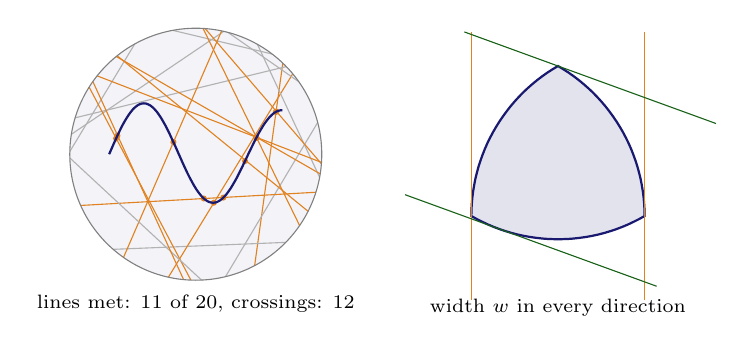
\begin{tikzpicture}[font=\scriptsize]
\begin{scope}\clip (0,0) circle (1.6);
\fill[MidnightBlue!5] (0,0) circle (1.6);
\draw[BurntOrange!90!black,line width=0.4pt] (1.340,2.842) -- (0.513,-3.100);
\fill[BurntOrange!90!black] (1.017,0.538) circle (1.1pt);
\draw[gray!60,line width=0.4pt] (2.503,1.999) -- (-0.577,-3.151);
\draw[gray!60,line width=0.4pt] (3.044,-1.043) -- (-2.951,-1.285);
\draw[gray!60,line width=0.4pt] (1.874,2.585) -- (-3.098,-0.772);
\draw[gray!60,line width=0.4pt] (3.257,0.727) -- (-2.579,2.118);
\draw[BurntOrange!90!black,line width=0.4pt] (2.007,2.290) -- (-1.123,-2.830);
\fill[BurntOrange!90!black] (0.229,-0.616) circle (1.1pt);
\draw[gray!60,line width=0.4pt] (2.724,1.495) -- (-3.107,0.080);
\draw[gray!60,line width=0.4pt] (0.363,3.285) -- (-2.738,-1.851);
\draw[BurntOrange!90!black,line width=0.4pt] (2.025,-2.348) -- (-0.614,3.040);
\fill[BurntOrange!90!black] (0.769,0.209) circle (1.1pt);
\draw[gray!60,line width=0.4pt] (2.450,-2.166) -- (-0.094,3.269);
\draw[BurntOrange!90!black,line width=0.4pt] (2.813,-1.537) -- (-1.099,3.012);
\fill[BurntOrange!90!black] (1.023,0.541) circle (1.1pt);
\draw[gray!60,line width=0.4pt] (3.321,-0.481) -- (-1.602,2.948);
\draw[BurntOrange!90!black,line width=0.4pt] (3.027,-0.399) -- (-2.963,-0.735);
\fill[BurntOrange!90!black] (0.102,-0.562) circle (1.1pt);
\fill[BurntOrange!90!black] (0.350,-0.551) circle (1.1pt);
\draw[BurntOrange!90!black,line width=0.4pt] (2.540,-1.632) -- (-2.112,2.157);
\fill[BurntOrange!90!black] (0.626,-0.087) circle (1.1pt);
\draw[BurntOrange!90!black,line width=0.4pt] (2.885,-1.001) -- (-2.315,1.992);
\fill[BurntOrange!90!black] (0.769,0.209) circle (1.1pt);
\draw[BurntOrange!90!black,line width=0.4pt] (0.691,-3.027) -- (-2.107,2.280);
\fill[BurntOrange!90!black] (-1.012,0.200) circle (1.1pt);
\draw[BurntOrange!90!black,line width=0.4pt] (0.898,2.881) -- (-1.487,-2.625);
\fill[BurntOrange!90!black] (-0.284,0.154) circle (1.1pt);
\draw[gray!60,line width=0.4pt] (1.437,-2.863) -- (-2.963,1.217);
\draw[BurntOrange!90!black,line width=0.4pt] (0.519,-3.062) -- (-1.980,2.392);
\fill[BurntOrange!90!black] (-0.995,0.236) circle (1.1pt);
\draw[BurntOrange!90!black,line width=0.4pt] (2.971,-0.634) -- (-2.627,1.525);
\fill[BurntOrange!90!black] (0.769,0.209) circle (1.1pt);
\end{scope}
\draw[gray] (0,0) circle (1.6);
\draw[MidnightBlue,thick] (-1.100,0.000) -- (-1.072,0.064) -- (-1.045,0.126) -- (-1.017,0.188) -- (-0.990,0.248) -- (-0.962,0.305) -- (-0.935,0.360) -- (-0.907,0.411) -- (-0.879,0.458) -- (-0.852,0.500) -- (-0.824,0.538) -- (-0.797,0.571) -- (-0.769,0.598) -- (-0.742,0.619) -- (-0.714,0.634) -- (-0.686,0.643) -- (-0.659,0.646) -- (-0.631,0.643) -- (-0.604,0.633) -- (-0.576,0.618) -- (-0.549,0.597) -- (-0.521,0.569) -- (-0.493,0.537) -- (-0.466,0.499) -- (-0.438,0.457) -- (-0.411,0.410) -- (-0.383,0.360) -- (-0.356,0.306) -- (-0.328,0.249) -- (-0.301,0.190) -- (-0.273,0.129) -- (-0.245,0.068) -- (-0.218,0.006) -- (-0.190,-0.056) -- (-0.163,-0.118) -- (-0.135,-0.178) -- (-0.108,-0.236) -- (-0.080,-0.292) -- (-0.052,-0.344) -- (-0.025,-0.393) -- (0.003,-0.439) -- (0.030,-0.479) -- (0.058,-0.515) -- (0.085,-0.546) -- (0.113,-0.572) -- (0.141,-0.592) -- (0.168,-0.606) -- (0.196,-0.614) -- (0.223,-0.616) -- (0.251,-0.613) -- (0.278,-0.603) -- (0.306,-0.588) -- (0.334,-0.567) -- (0.361,-0.540) -- (0.389,-0.509) -- (0.416,-0.472) -- (0.444,-0.432) -- (0.471,-0.387) -- (0.499,-0.339) -- (0.527,-0.288) -- (0.554,-0.234) -- (0.582,-0.178) -- (0.609,-0.121) -- (0.637,-0.063) -- (0.664,-0.005) -- (0.692,0.053) -- (0.720,0.110) -- (0.747,0.166) -- (0.775,0.219) -- (0.802,0.271) -- (0.830,0.319) -- (0.857,0.364) -- (0.885,0.405) -- (0.913,0.442) -- (0.940,0.474) -- (0.968,0.501) -- (0.995,0.524) -- (1.023,0.541) -- (1.050,0.552) -- (1.078,0.558) -- (1.100,0.559);
\fill[MidnightBlue!12,draw=MidnightBlue,thick] (3.500,-0.785) -- (3.570,-0.824) -- (3.640,-0.859) -- (3.712,-0.893) -- (3.786,-0.924) -- (3.860,-0.952) -- (3.935,-0.977) -- (4.011,-1.000) -- (4.088,-1.020) -- (4.166,-1.037) -- (4.244,-1.051) -- (4.323,-1.062) -- (4.402,-1.071) -- (4.481,-1.077) -- (4.560,-1.079) -- (4.640,-1.079) -- (4.719,-1.077) -- (4.798,-1.071) -- (4.877,-1.062) -- (4.956,-1.051) -- (5.034,-1.037) -- (5.112,-1.020) -- (5.189,-1.000) -- (5.265,-0.977) -- (5.340,-0.952) -- (5.414,-0.924) -- (5.488,-0.893) -- (5.560,-0.859) -- (5.630,-0.824) -- (5.700,-0.785) -- (5.700,-0.785) -- (5.699,-0.706) -- (5.694,-0.626) -- (5.687,-0.547) -- (5.677,-0.468) -- (5.664,-0.390) -- (5.649,-0.312) -- (5.630,-0.235) -- (5.609,-0.158) -- (5.585,-0.083) -- (5.558,-0.008) -- (5.529,0.066) -- (5.497,0.139) -- (5.462,0.210) -- (5.425,0.280) -- (5.385,0.349) -- (5.343,0.416) -- (5.298,0.482) -- (5.251,0.546) -- (5.202,0.609) -- (5.151,0.669) -- (5.097,0.728) -- (5.042,0.785) -- (4.984,0.839) -- (4.924,0.892) -- (4.863,0.942) -- (4.800,0.990) -- (4.735,1.036) -- (4.668,1.079) -- (4.600,1.120) -- (4.600,1.120) -- (4.532,1.079) -- (4.465,1.036) -- (4.400,0.990) -- (4.337,0.942) -- (4.276,0.892) -- (4.216,0.839) -- (4.158,0.785) -- (4.103,0.728) -- (4.049,0.669) -- (3.998,0.609) -- (3.949,0.546) -- (3.902,0.482) -- (3.857,0.416) -- (3.815,0.349) -- (3.775,0.280) -- (3.738,0.210) -- (3.703,0.139) -- (3.671,0.066) -- (3.642,-0.008) -- (3.615,-0.083) -- (3.591,-0.158) -- (3.570,-0.235) -- (3.551,-0.312) -- (3.536,-0.390) -- (3.523,-0.468) -- (3.513,-0.547) -- (3.506,-0.626) -- (3.501,-0.706) -- (3.500,-0.785) -- cycle;
\draw[BurntOrange!90!black] (3.500,-1.850) -- (3.500,1.550);
\draw[BurntOrange!90!black] (5.700,-1.850) -- (5.700,1.550);
\draw[ForestGreen!70!black] (5.853,-1.677) -- (2.658,-0.514);
\draw[ForestGreen!70!black] (6.606,0.390) -- (3.411,1.553);
\node at (4.6,-1.95) {width $w$ in every direction};
\node at (0,-1.9000000000000001) {lines met: 11 of 20, crossings: 12};
\end{tikzpicture}
